\chapter{Examples}

\section{Introduction}
The 1D-3C SEM code is served to use with several examples which had been used in analyses of \cite{Oral2016}. First, for an elastic medium assumption, the realistic model of Volvi (Greece) is given. Second, the same model of Volvi is used with viscoelastic soil constitutive model. Afterwards, nonlinear examples are shown for different cases. One of the nonlinear cases is the pressure-independent P1 model. The soil nonlinearity in this model is considered by elastoplasticity where 50 Iwan mechanisms are defined. Another nonlinear case is the pressure-dependent model of Wildlife Refuge Liquefaction Array (WRLA) which is provided with total and effective stress analyses. Lastly, effective stress analysis of Kushiro port (KP) site model which is initially anisotropically consolidated is provided. These examples are detailed by input and output files below.\\


\section{Elasticity model}

For elasticity, Volvi model example is given. It can be found in EXAMPLES\slash VOLVI\slash ELASTIC directory. The model is composed of eight soil layers. In the table below, main properties of the model are shown, where $\rho$ is soil density, $V_{s}$ and $V_{p}$ are shear and pressure wave velocities, $Q_{s}$ and $Q_{p}$ are quality factors for shear and pressure waves, respectively. For elasticity, $Q_{s}$ and $Q_{p}$ values are ignored. \\


\vspace{1cm}
% Table : Volvi soil ppts
\captionof{table}{Soil properties at the Volvi model.}
\label{TABvolvi}
\begin{center}
\begin{tabular}{|c|c|c|c|c|c|c|c|} \hline                                
Layer  & Thickness $[m]$ & $V_{s} [m/s] $ &  $V_{p} [m/s] $   & $\rho [kg/m^{3}]$ & $Q_{s}$& $Q_{p}$  \\ \hline \hline 
1     & 7    	& 130 	& 1500  & 2050   &  15 	  & 75  \\ \hline    
2     & 13     	& 200   & 1500	& 2150   &  20    & 75  \\ \hline    
3     & 34    	& 300   & 1650	& 2075   &  30    & 83  \\ \hline    
4     & 23.5    & 450   & 2050	& 2100   &  40    & 103 \\ \hline    
5     & 50    	& 600   & 2450	& 2155   &  60    & 123	\\ \hline    
6     & 59    	& 700   & 2550	& 2200   &  70    & 140	 \\ \hline    
7     & 10    	& 1250  & 3500	& 2500   &  100   & 200  \\ \hline    
Bedrock& 103.5  & 2600  & 4500	& 2600   &  50000 & 50000 \\ \hline    
\end{tabular}
\end{center}

In this example, upper boundary is defined as free surface and at bottom of the model, PML (Perfectly Matched Layers) is used. It should be noted that 1D-3C SEM code assumes use of a single element for PML. For further changes, the user could make modifications  in the code by ‘sigeps.f90’ file. \\


The first file that the user should provide is ‘input.spec’, which is shown in the following figure of Volvi model. \\

% FIGURE : INPUT.SPEC
\begin{center}
\leavevmode
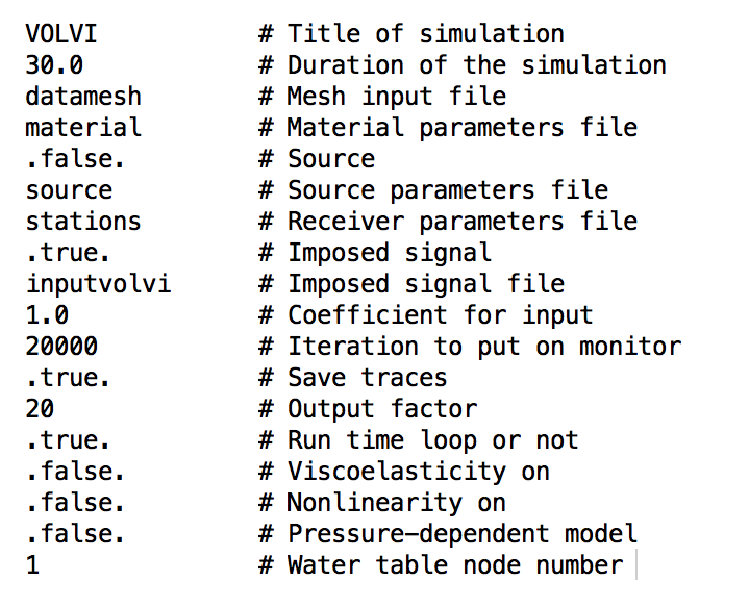
\includegraphics [scale=0.75] {figures/inputspec.eps} 
\label{inputspec} 
\captionof{figure}{Input file input.spec for elastic Volvi model.}
\vspace{1cm}
\end{center}


The file is self-explanatory. Title of simulation and total duration of simulation should be specified. Then, the mesh file name from which the necessary data about element and domain characteristics are to be read is needed. In pre-treatment section of this manual, an example for creating a mesh file is given. \\

For material properties, the code requires a file which respects the following format. The user should define total number of domains. Then , for each domain, P and S velocity values, density, PML condition (True \slash False), time step of simulation, GLL number, viscoelasticity quality factors for P and S waves, reference frequency and nonlinear soil type should be written. Although same time step is used all over the model, the format requires entering this data for each domain. For elastic models, even though it is not necessary viscoelastic or nonlinear parameters in computations, the user should follow the specified format for every model. For PML domain, n and A coefficients are necessary.  If no PML is used, the PML data section should be left commented. Lastly, for pressure-dependent models, for each domain, the user must define whether excess pore pressure development is expected (T) or not (F) and pressure-dependent soil type. In other models such as this elastic example, this part will be ignored. However, the user should create the material file in this format. \\

% FIGURE : MATERIAL
\begin{center}
\leavevmode
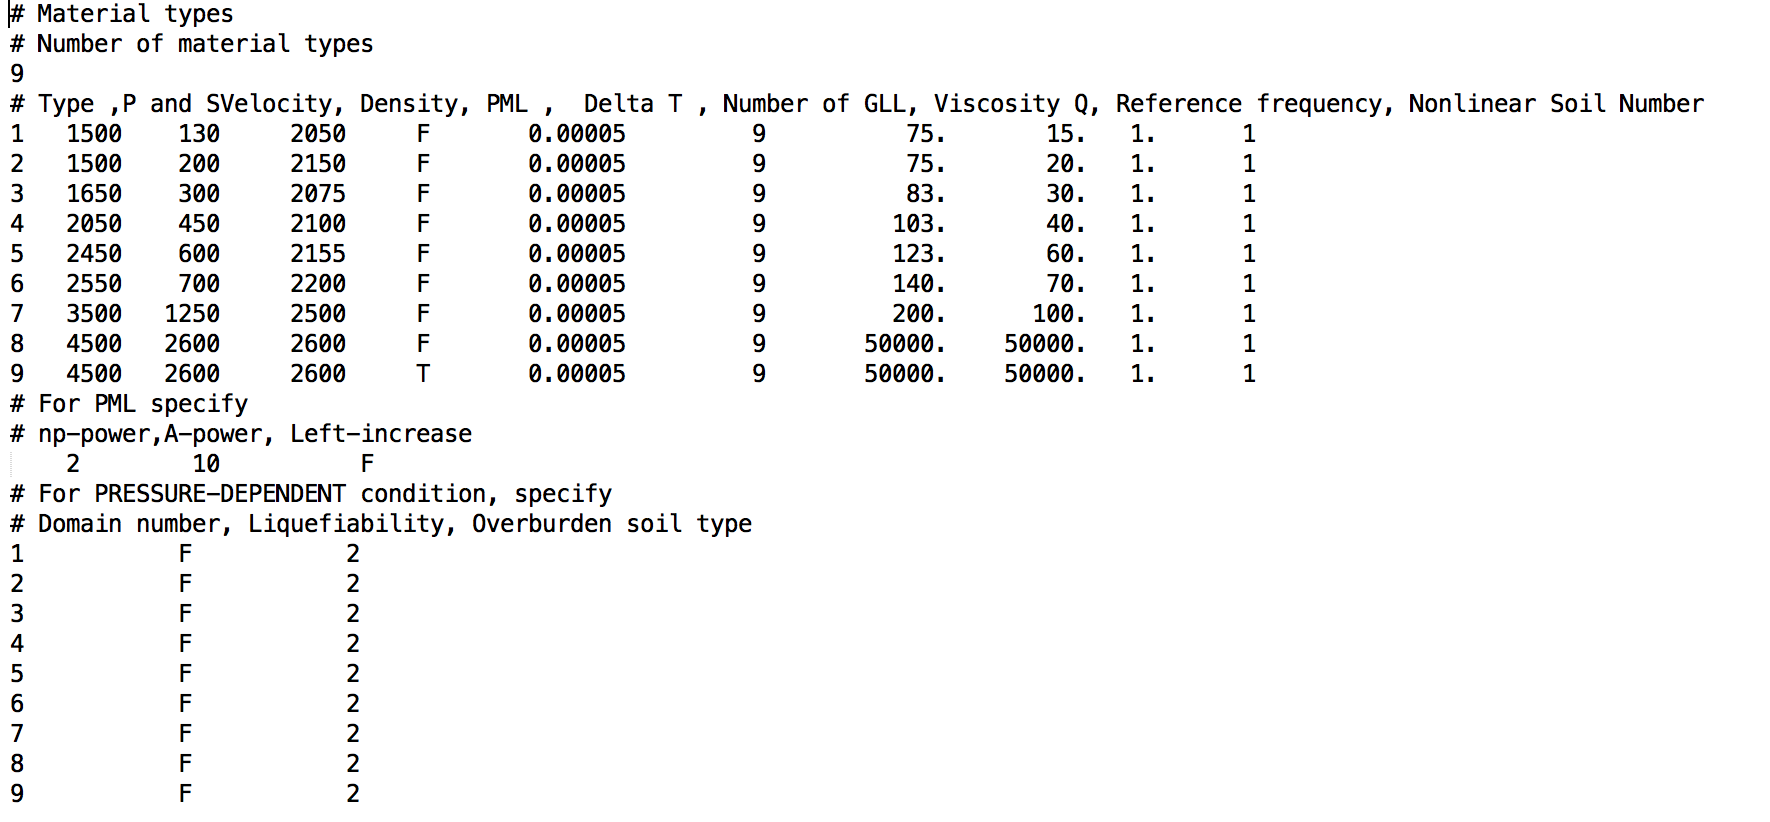
\includegraphics [scale=0.6] {figures/material.eps} 
\captionof{figure}{Material file for elastic Volvi model.}
\label{mat} 
\vspace{1cm}
\end{center}


When we come back to input file, the following input data concerns sources. For cases where point source is defined as input motion, the user should set source option should be defined as ‘.True.’ and specify file name in which source type and properties are given . Such a source file should contain: \\

\begin{enumerate}

\item Coordinate
\item Source kind (1 for impulse; 2 for explosion)
\item Source function (1 for Gaussian; 2 for Ricker)
\item Pulse width (Only if Gaussian type of function is given)
\item Delay time  (Only if Ricker type of function is given)
\item Cut-off frequency (Only if Ricker type of function is given)

\end{enumerate}


For cases where the input motion is defined by an incident wave field, the code requires a file in which time step and corresponding velocity of incident wave are included. It should be noted that time step of the input motion should not be smaller than time step of simulation. For such cases, the user should write ‘.True.’ for imposed signal and file name for imposed signal file. It is also possible to define a coefficient for the given velocity field. \\

The receiver coordinates should be included in a file with total number of stations. An example is given below: \\

% FIGURE : STATIONS
\begin{center}
\leavevmode
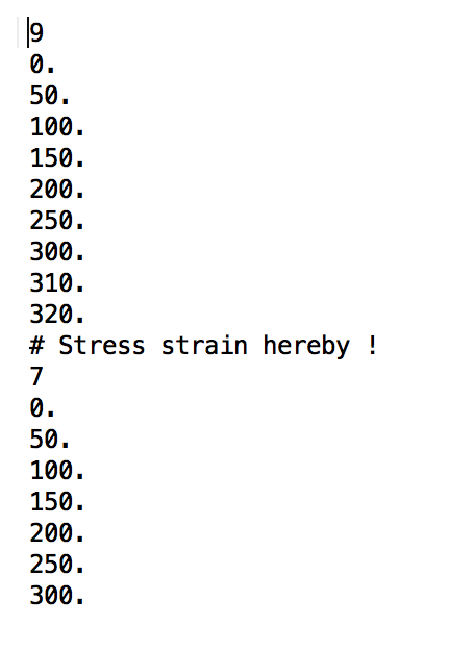
\includegraphics [scale=0.75] {figures/stations.eps} 
\captionof{figure}{Station (receiver) file for elastic Volvi model.}
\label{stat} 
\vspace{1cm}
\end{center}

In receiver file (‘stations’ in this example), first, the receivers where acceleration, velocity time histories are desired as output are defined. In the second part of the file, different depths could be defined for saving nonlinearity and pore pressure model parameters. More details about output files are given in last chapter of this manual (See Chapter \ref{sec:prepost}). \\

When the code is executed, some information are written out in terminal as below : \\

% FIGURE : TERMINAL
\begin{center}
\leavevmode
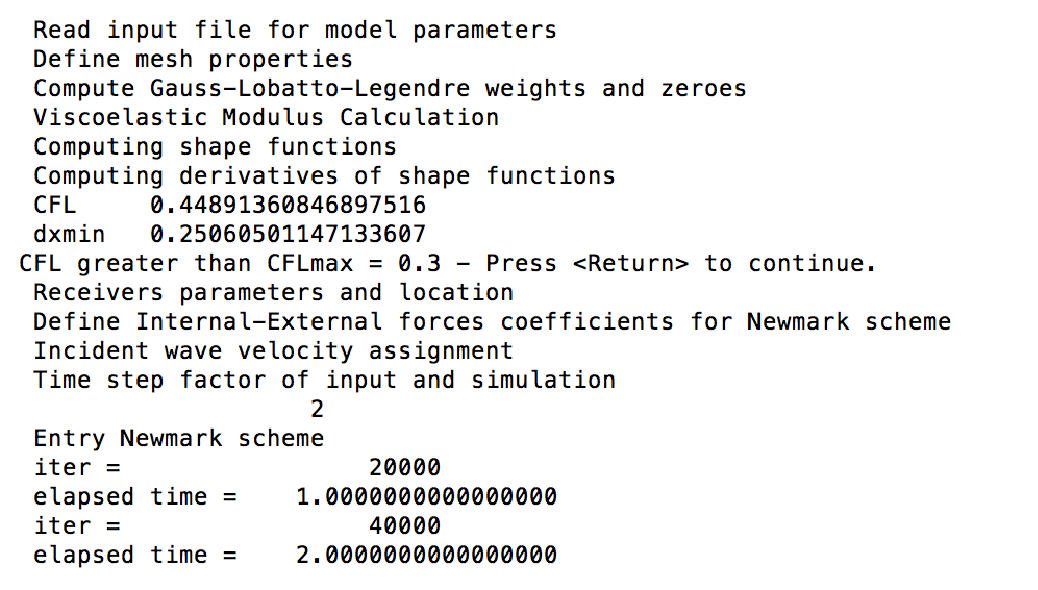
\includegraphics [scale=0.75]{figures/terminal.eps} 
\captionof{figure}{Output data in terminal for 2 seconds of simulation in elastic Volvi model.}
\label{ter} 
\vspace{1cm}
\end{center}


In order to control the time interval of output information concerning elapsed time, the user could change the iteration number in input.spec file by ‘iteration to put on monitor’. For the simulations where the user does not want to perform time iterations but verifies the execution of the code (useful for further modifications by advanced users), ‘Run time loop’ could be chosen as ‘.False.’. Also, if the user does not want to save output files, ‘Save traces’ should be chosen as False. Otherwise, at the end of simulation, the code provides output files at given receiver coordinates. \\

Lastly, the soil constitutive models should be defined. For elasticity, the user should set ‘Viscoelasticity on’, ‘Nonlinearity on’ and ‘Pressure-dependent model’ False. The other cases will be detailed in following sections. For elasticity, ‘Water table node’ is not taken into consideration in computations. \\



\section{Viscoelasticity model}

Viscoelasticity example could be found in EXAMPLES\slash VOLVI\slash VISCOELASTIC directory.  For viscoelasticity, compared to elasticity, the changes apply to input.spec and material files. In input.spec files, differently than elasticity, ‘Viscoelasticity on’ should be set to ‘True’. In material file, quality factors for P and S waves with reference frequency (which will be no longer ignored by the code) should be provided for each domain. 


\section{Nonlinearity model}

\subsection{Pressure-independent nonlinearity}

For pressure-independent nonlinear model, an example is given in EXAMPLES\slash P1 directory.  The model is composed of a single layer with following properties: \\

\vspace{1 cm}
% Table : WL soil ppts
\captionof{table}{Soil properties at P1 model (PRENOLIN).}
\label{tabP1}
\begin{center}
\begin{tabular}{|c|c|c|c|c|c|c|} \hline                                
Layer & Thickness $[m]$ & $V_{s} [m/s] $ &$V_{p} [m/s] $ & $\rho [kg/m^{3}]$ & $Q_{s}$ & $Q_{p}$ \\ \hline \hline 
1     &  20   		& 300  		& 700 		&  2000 	     & 30  & 70  \\ \hline    
\end{tabular}
\end{center}


In such a case, the user should define, first, in input.spec file, ‘Nonlinearity on’ as True, so that the model follows elastoplasticity. If viscous attenuation is also demanded, then ‘Viscoelasticity on’ must be set to True as well, such that the model is visco-elastoplastic. \\

Also, for nonlinearity, another file which should be named ‘GoverGmax.dat’ is required, differently than elastic and viscoelastic cases. The format of the file is shown below: \\

% FIGURE : GoverGmax.dat
\begin{center}
\leavevmode
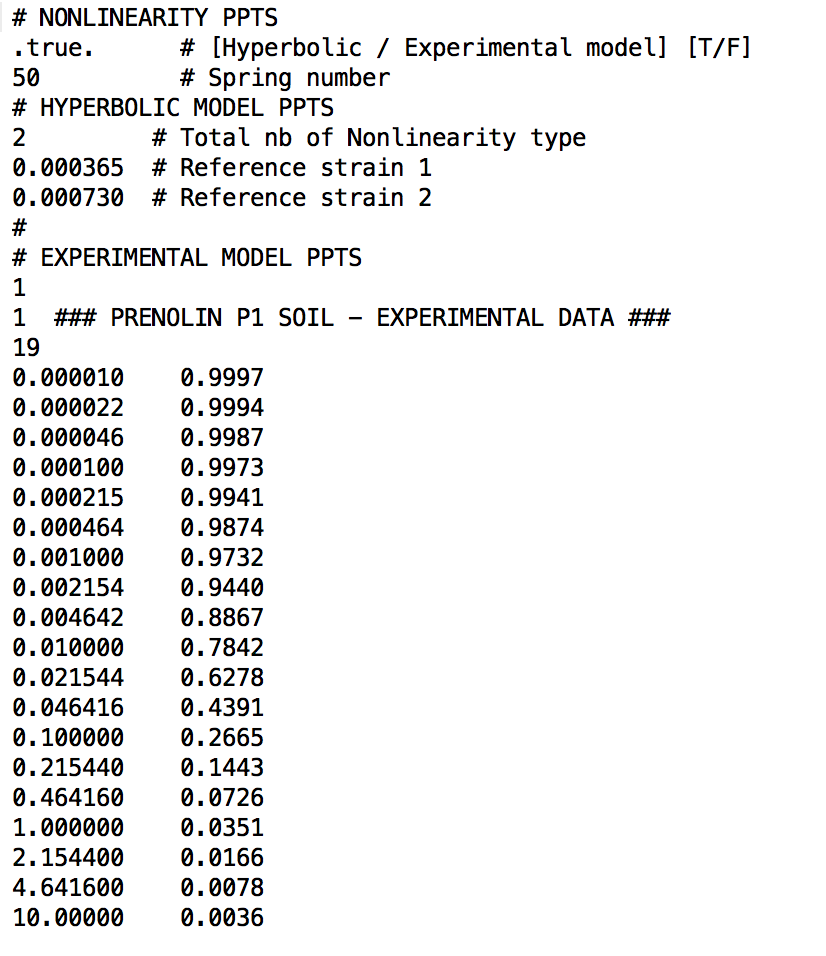
\includegraphics [scale=0.75] {figures/GoverGmaxdat.eps} 
\captionof{figure}{GoverGmax.dat file for P1 example.}
\label{GG} 
\vspace{1cm}
\end{center}

In this latter, the choice of hyperbolic or experimental model in order to construct the backbone curve should be made. For hyperbolic models, the Equation \ref{eqHD} is used so that the user must define a reference strain. \\


% Equation - Hardin and Drnevich 1972
\begin{equation}
\label{eqHD}
\frac{G}{G_{0}} = \frac{1}{1+ \gamma / \gamma_{ref}} 
\end{equation}


In this example, two different values are available. In ‘material’ file, the nonlinear soil type should be written according to the reference strain data in this file, for hyperbolic models. Otherwise, the user has the possibility of defining an experimental curve by giving strain (in percentage) and corresponding shear modulus ratio. Again, the soil type must match with the defined nonlinear soil type in ‘material’ file for each domain. Lastly, in the same file, the total number of Iwan springs is obligatorily given for all nonlinear cases. In this example, it is set to 50. \\


\subsection{Pressure-dependent nonlinearity}

For pressure-dependent model, Wildlife Refuge Liquefaction Array site model is given.  The model is composed of four layers of which only the third layer is liquefiable. In other words, only in the third layer, excess pore pressure development is expected to be developed. \\



% Table : WL soil ppts
\captionof{table}{Soil properties at Wildlife Refuge Liquefaction Array after \protect\cite{Bonilla2005} }
\begin{center}
\begin{tabular}{|c|c|c|c|c|c|c|c|} \hline                                
Layer & Description  & Thickness $[m]$ & $V_{s} [m/s] $ &$V_{p} [m/s] $ & $\rho [kg/m^{3}]$ & $\phi_{f} [degree]$ & $K_{0}$ \\ \hline \hline 
1     & Silt    		& 1.5   & 99  & 249 &  1600 & 28  & 1.0  \\ \hline    
2     & Silt    		& 1.0   & 99  & 281 &  1928 & 28  & 1.0  \\ \hline
3     & Silty sand 	& 4.3   & 116 & 1019&  2000 & 32  & 1.0  \\ \hline
4     & Silty sand 	& 0.7   & 116 & 1591&  2000 & 32  & 1.0  \\ \hline
\end{tabular}
\label{TAB:WRLA1}
\end{center}



For this site, the models of effective and total stress analyses are provided. First, necessary modifications for total stress analysis are detailed. Then, further changes to be made for effective stress analysis are explained. \\

\paragraph{Total stress analysis}

For total stress analysis, in other words, for pressure-dependent nonlinear models where no excess pore pressure develops, the first change applies to ‘input.spec’ file. The user should define ‘Nonlinearity on’ and ‘Pressure-dependent model’ as True. The water level should be defined by the corresponding node number in mesh file. This means that if water level is present in the model, it must correspond to an elementary boundary in the model.  \\

In addition, differently than previous cases, in pressure-dependent model, another file ‘pressparam.dat’ is required. The format of the file is given below.  In this file, m1 (slope of the soil failure line), cohesion and coefficient of Earth at rest are compulsory for total stress analysis. Other parameters are to be neglected in total stress analysis computations. \\

%% FIGURE : pressparam.dat
\begin{center}
\leavevmode
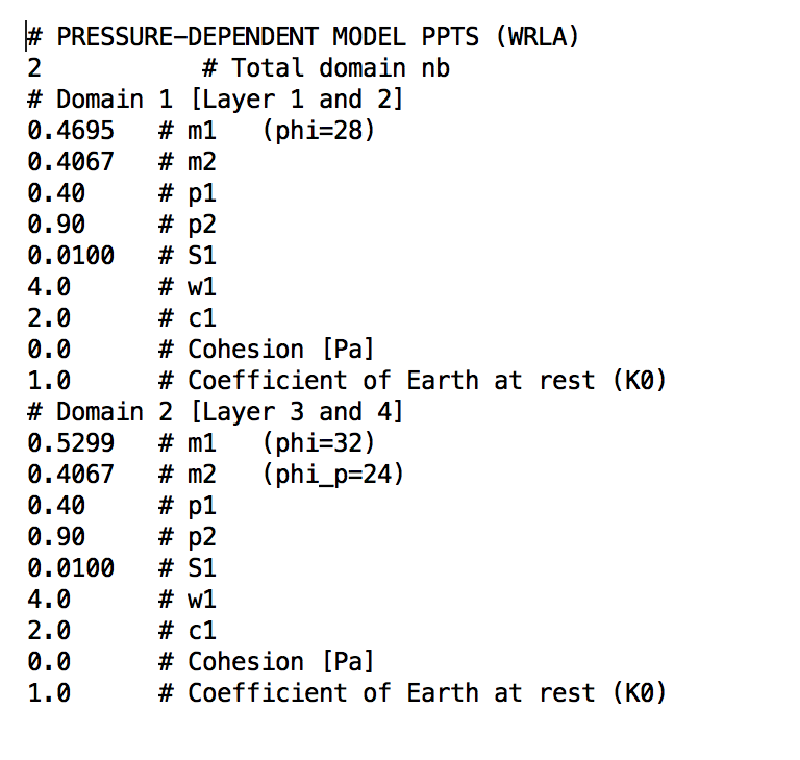
\includegraphics [scale=0.75] {figures/pressparamdat.eps} 
\captionof{figure}{pressparam.dat file for P1 example.}
\label{press} 
\vspace{1cm}
\end{center}


Accordingly, in the last part of the material file, the overburden soil type should match the soil number in ‘pressparam.dat’ soil types. For total stress analysis, each domain is non-liquefiable such that liquefiability is specified as False. \\


\paragraph{Effective stress analysis}

Effective stress analysis for WRLA model can be found in EXAMPLES\slash WRLA\slash EFFECTIVE \textunderscore STRESS\textunderscore ANALYSIS directory. In WRLA model, the third layer is assumed to be liquefiable. This property is defined in the liquefiability part of the material file. For this example, the third layer liquefiability is True while other layers are False, as seen in Figure \ref{matwrla}. 


% FIGURE : MATERIAL WRLA
\begin{center}
\leavevmode
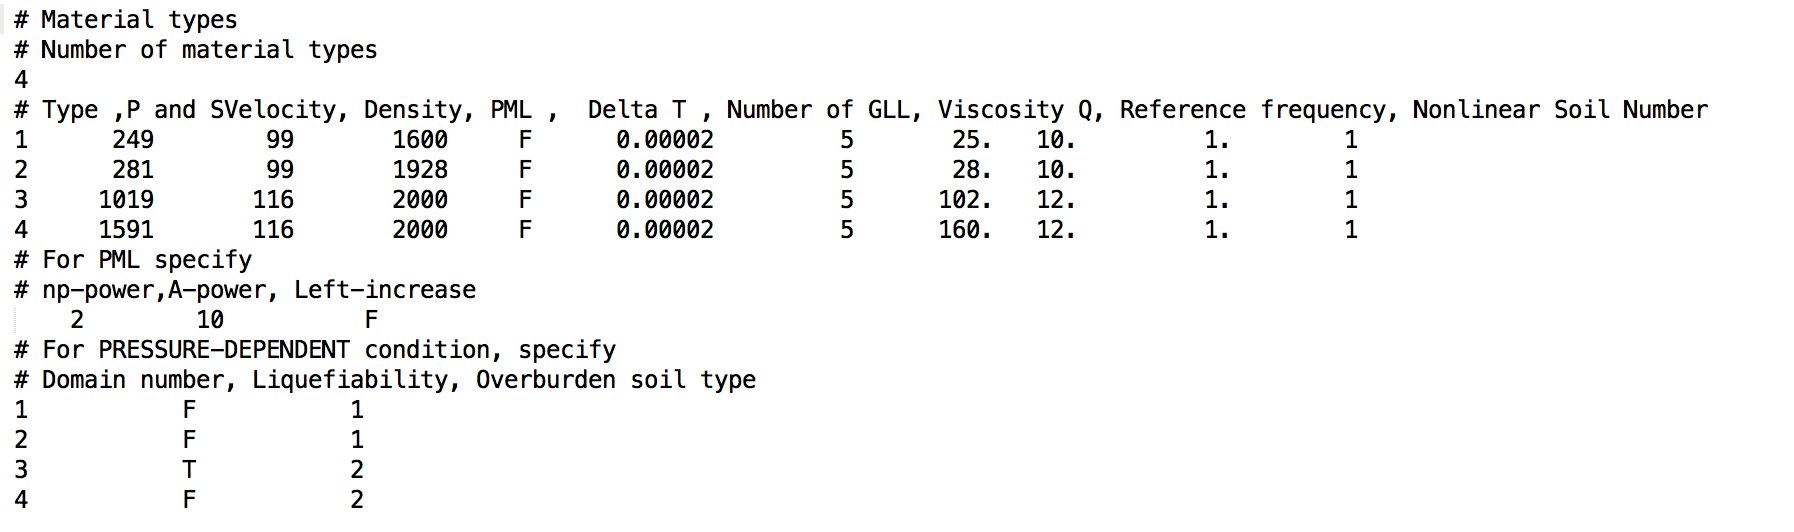
\includegraphics[scale=0.6]{figures/mat2.eps} 
\captionof{figure}{Material file for WRLA effective stress analysis model.}
\label{matwrla} 
\vspace{1cm}
\end{center}

Compared to total stress analysis, another change is made in pressparam.dat file. The model properties necessary for pore pressure excess computation such as $m_{2}$, $p_{1}$, $p_{2}$, $S_{1}$ and $w_{1}$ (front saturation model parameters) are required for the liquefiable layer. In this example, the third layer corresponds to the  overburden soil type 2. Thus, in pressparam.dat file, the code looks for the front saturation model parameters for that soil type. 

\paragraph{Effective stress analysis - II}

Another example is given for effective stress analysis in Kushiro Port model (KP), which is initially consolidated in anisotropic conditions. The KP model properties are given in Table \ref{KUSH2}. \\


\vspace{1cm}
% Table : KP soil ppts
\captionof{table}{Soil properties at Kushiro Port vertical array after \protect\cite{Iai1995}. $V_{p}$ values are calculated by assumption of Poisson ratio equal to $0.48$. }
\begin{center}
\begin{tabular}{|c|c|c|c|c|c|c|c|} \hline                                
Layer & Description  & Thickness $[m]$ & $V_{s} [m/s] $ &$V_{p} [m/s] $ & $\rho [kg/m^{3}]$ & $\phi_{f} [degree]$ & $K_{0}$ \\ \hline \hline 
1     & Fill soil    	& 2.0    	& 249  & 1270 	&  1540 & 40 & 0.5  \\ \hline    
2     & Sand    	& 7.0    	& 249  & 1270	&  1720 & 40 & 0.5  \\ \hline
3     & Sand	 	& 14.0   	& 326  & 1662 	&  1980 & 48 & 0.5  \\ \hline
4     & Silt 		& 9.0    	& 265  & 1351 	&  1730 & 37 & 0.5  \\ \hline
5     & Silt 		& 4.0    	& 341  & 1739 	&  1760 & 44 & 0.5  \\ \hline
6     & Silt 		& 8.0    	& 286  & 1458 	&  1700 & 44 & 0.5  \\ \hline
7     & Silt 		& 8.0    	& 302  & 1540 	&  2000 & 45 & 0.5  \\ \hline
8     & Silt 		& 25.0   	& 341  & 1739 	&  1730 & 44 & 0.5  \\ \hline
\end{tabular}
\label{KUSH2}
\end{center}


Since the model has a coefficient of Earth at rest equal to 0.5 for each layer, this property is defined in ‘pressparam.dat’ file with K0 parameter. \\
